%%%%%%%%%%%%%%%%%%%%%%%%%%%%%%%%%%%%%%%%%
% University/School Laboratory Report
% LaTeX Template
% Version 4.0 (March 21, 2022)
%
% This template originates from:
% https://www.LaTeXTemplates.com
%
% Authors:
% Vel (vel@latextemplates.com)
% Linux and Unix Users Group at Virginia Tech Wiki
%
% License:
% CC BY-NC-SA 4.0 (https://creativecommons.org/licenses/by-nc-sa/4.0/)
%
%%%%%%%%%%%%%%%%%%%%%%%%%%%%%%%%%%%%%%%%%

%----------------------------------------------------------------------------------------
%	PACKAGES AND DOCUMENT CONFIGURATIONS
%----------------------------------------------------------------------------------------

\documentclass[
	letterpaper, % Paper size, specify a4paper (A4) or letterpaper (US letter)
	10pt, % Default font size, specify 10pt, 11pt or 12pt
]{CSUniSchoolLabReport}

\addbibresource{references.bib} % Bibliography file (located in the same folder as the template)

%----------------------------------------------------------------------------------------
%	REPORT INFORMATION
%----------------------------------------------------------------------------------------

\title{\textbf{Reinforcement Learning for Bomberman \\ Final Project}} % Report title

\author{Angelina Basova \\ Tobias Neuschäfer \\Sven Zelch} % Author name(s), add additional authors like: '\& James \textsc{Smith}'

\date{\today} % Date of the report

%----------------------------------------------------------------------------------------

\begin{document}
\maketitle % Insert the title, author and date using the information specified above

\begin{center}
	\begin{tabular}{l r}
		Tutor:      & TODO                     \\
		Instructor: & \textsc{Ullrich K\"othe} % Instructor/supervisor
	\end{tabular}
\end{center}



\newpage

\tableofcontents
\newpage

\listoffigures
\listoftables
\newpage

% If you need to include an abstract, uncomment the lines below
%\begin{abstract}
%	Abstract text
%\end{abstract}

%----------------------------------------------------------------------------------------
%	INTRODUCTION
%----------------------------------------------------------------------------------------

\section{Introduction}

%----------------------------------------------------------------------------------------
%	METHODS
%----------------------------------------------------------------------------------------

\section{Methods}

\subsection{Q-Learning}
\subsection{Reward Shaping}

%----------------------------------------------------------------------------------------
%	TRAINING
%----------------------------------------------------------------------------------------

\section{Training}
\subsection{Q-Learning}

\subsubsection*{Q Table}
A major challenge to implement Q-Learning was the creation of a feature space.
We initialize the Q table as a dictionary, whose keys are the features and the values are the values of the Q function for the six
actions.
Choosing a dictionary as the preferred data structure for the Q table provided us
two major benefits.
First, we we were able to increase its size and thus its feature space flexibly.
This proved to be quite helpful to derive training strategies because we
could focus on the q values of almost the same states.
Additionally, we didn't feel the need to create a Q table covering every possible
feature space as for unseen states, we picked actions from a similar seen state.

\subsubsection*{Feature space}
Our features consist of ten values. The majority of the values contain the Manhattan distance between
the agent and the nearest object of interest. For instance, Figure \ref{fig:example} illustrates a possible feature.
The feature shows that the agent is only one cell away from a coin in the x-axis as the first value equals to one.
The y value equals to 0, which means that the agent is in the same row as the coin.


\begin{center}
	\begin{figure}[H]
		\scalebox{0.7}{
			\begin{tabular}{ccccccccccc}
				          &                                                        &         &       &        &                                                         & \multicolumn{2}{c}{
\includegraphics[width=1cm]{Figures/robot_pink.png}} &                              \\
				          & \multicolumn{2}{c}{
\includegraphics{Figures/coin.png}} &         &       &        & \multicolumn{2}{c}{
\includegraphics{Figures/crate.png}} & \multicolumn{2}{c}{
\includegraphics{Figures/bomb_blue.png}}                                            \\
				\\
				feature = & (coin x,                                               & coin y, & left, & right, & down,  up,                                              & crate x ,                                                               & crate y, & bomb x, & bomb y)
			\end{tabular}}
		\caption{Illustration of the feature structure encoding the space of the agent}
	\end{figure}
\end{center}


\begin{center}
	\begin{figure}[h]
		\centering
		\begin{tabular}{ccccccccccc}
			feature = & (1, & 0, & 0, & 0, & 1, & 1, & 5, & 1, & 9, & 12)
		\end{tabular}
		\caption{Example of a feature }
		\label{fig:example}
	\end{figure}
\end{center}



\subsubsection*{Auxilliary Rewards}
In order to incentivize the agent to perform beneficial actions we used a number of auxilliary rewards.
The rewards were split into five different categories, which indicate in which case the auxilliary reward
is earned. For instance, the auxilliary reward MOVED\_IN\_CYCLE corresponds to the general category. This
means that the reward can be earned at any step in the game. While the auxilliary reward MOVED\_TO\_CRATE can
only be earned when a crate or an opponent is present in the features, thus its category is Crates, Opponents.

\begin{table}[H]
	\centering
	\scalebox{0.8}{
		\begin{tabular}{llc}
			Category & Auxilliary Rewards          & Value \\
			\hline \hline
			\multirow{4}*{General}
			         & e.VALID\_ACTION             & 0     \\
			         & NOT\_VALID\_ACTION          & -2000 \\
			         & MOVED\_IN\_CYCLE            & -2000 \\
			         & NOT\_MOVED\_IN\_CYCLE       & 0     \\
			\hline
			\multirow{4}*{Coins}
			         & e.COIN\_COLLECTED           & 1000  \\
			         & e.COIN\_FOUND               & 20    \\
			         & MOVED\_TO\_COIN             & 50    \\
			         & MOVED\_AWAY\_FROM\_COIN     & -5    \\
			\hline
			\multirow{3}*{Crates, Opponents}
			         & e.DIDNT\_DROP\_BOMB         & -60   \\
			         & MOVED\_TO\_CRATE            & 100   \\
			         & MOVED\_AWAY\_FROM\_CRATE    & -50   \\
			\hline
			\multirow{8}*{Bombs}
			         & MOVED\_TO\_BOMB             & -2000 \\
			         & MOVED\_AWAY\_FROM\_BOMB     & 200   \\
			         & MEANINGFUL\_WAIT            & 5     \\
			         & NOT\_MEANINGFUL\_WAIT       & -30   \\
			         & SAFE\_FROM\_BOMB            & 200   \\
			         & NOT\_SAFE\_FROM\_BOMB       & -200  \\
			         & MEANINGFUL\_BOMB\_DROP      & 200   \\
			         & NOT\_MEANINGFUL\_BOMB\_DROP & -400  \\
			\hline
			\multirow{3}*{Life}
			         & e.KILLED\_SELF              & -2000 \\
			         & NOT\_KILLED\_SELF           & 0     \\
			         & e.KILLED\_OPPONENT          & 1000  \\
			         & e.OPPONENT\_ELIMINATES      & 50    \\
			         & e.GOT\_KILLED               & -2000 \\
			         & e.SURVIVER\_ROUND           & 0     \\
			\hline
		\end{tabular}}
	\caption{Auxilliary rewards and their values}
	\label{tab:rewards}

\end{table}



\subsubsection{Discussion}
The agent showed some promising results in specific circumstances. The following points discuss
some problems and solutions to improve the agent.

\paragraph*{Zero values}
A major bottleneck in the development of the agent was the lengthy training. The majority of
the last week before the submission was utilized for training. However, this proved to not be enough as 50\%
of the actions in the Q table contained a zero value, meaning that the action was never tried out.

\paragraph*{Better choice among zero values}
Based on the observed training per state, which equals to XX min /per XX rounds or games it wouldn't
be feasible to train the agent until it converges to a good policy. During training fine-grained
tasks such as the collection of coins, we observed that the agent showed acceptable performance
after the Q table passed the threshold of XX non-zero values. This indicates that after XX state-action pairs
were selected at least one, the Q table converged to a good policy.
When the threshold is reached, there are XX zero values in the Q table or in other words, XX state-action pairs not
tried out yet. In certain states, the tried out actions contained negativ Q values. This drove the agent to
choose one of the not tried out actions, as their value of zero is higher than any negative value.
In this case, the agent would choose the first zero valued action. An interesting adjustment, would
be to choose a random action of the zero valued. This would provide two major benefits.

1. As during axploration, we choose the first zero valued action to try, we can see that the
majority of the first actions have been tried out, while the majority of the last two actions contain the most zero values.
This drove the agent to choose the last two actions, 'WAIT' and 'BOMB', the majority of the time
when tried out actions of the current state contained a negative Q value.

\paragraph*{Decision time at unseen states}
\paragraph*{Similar states}
A major problem that we oversaw was that the agent needed more time than specified to choose an action.
This was the case, when the agent was in a state, that wasn't present in the Q table. In out implementation, we
choose an action from the most similar state present in the Q table. We define state similarity as a weighted euclidean
distance. Our weight vector $w$ is $ w= (3, 3, 2, 2, 2, 2, 1, 1, 4, 4)$. The weights were
chosen based on the winning criteria of the game. As the winner is the agent with the highest score,
we chose the highest weight of 4 for the nearest bomb distance following with a weight of 3 for the nearest coin distance.
Next, we felt that a similar state should contain the same free tiles as the unseen state, to avoid invalid actions to be chosen.
Finally, we believe that the distance to a crate or opponent is not crucial for an unseen state as they don't influence the agent't score directly.
Thus we chose a weight of 1.

\paragraph*{Computation of similar states}
To compute a similar state we used an efficient function provided by the scipy library. We
tested the implementation of fine-grained tasks and always determined the best action
whithin the given time frame. However, the final submitted agent exceeded think time in multiple time steps of every round.
The reasons is that we iterated over all states of the Q table to compute the euclidean distance between
the current state. As the Q table increased dramatically in size once we merged the three tables, the iteration took longer than the provided
think time for the agent. A better approach would be to use another more efficient function provided by scipy
that handles the iteration internally.




%----------------------------------------------------------------------------------------
%	EXPERIMENTS
%----------------------------------------------------------------------------------------

\section{Experiments and Results}

\subsection{Q-Learning}
The submitted agent exceeds the majority of the think time due to an iteration while searching for
similar states.
As the exceeding in think time isn't related to Q-Learning but to the programmatic implementation of a search function,
we perform the following experiments after replacing the iteration with a scipy function.
The result of the search function remains the same.
However, this way we are able to illustrate the performance of our Q-Learning implementation
considerating the selected hyperparameters and auxilliary rewards.


\begin{figure}[h]
	\centering
	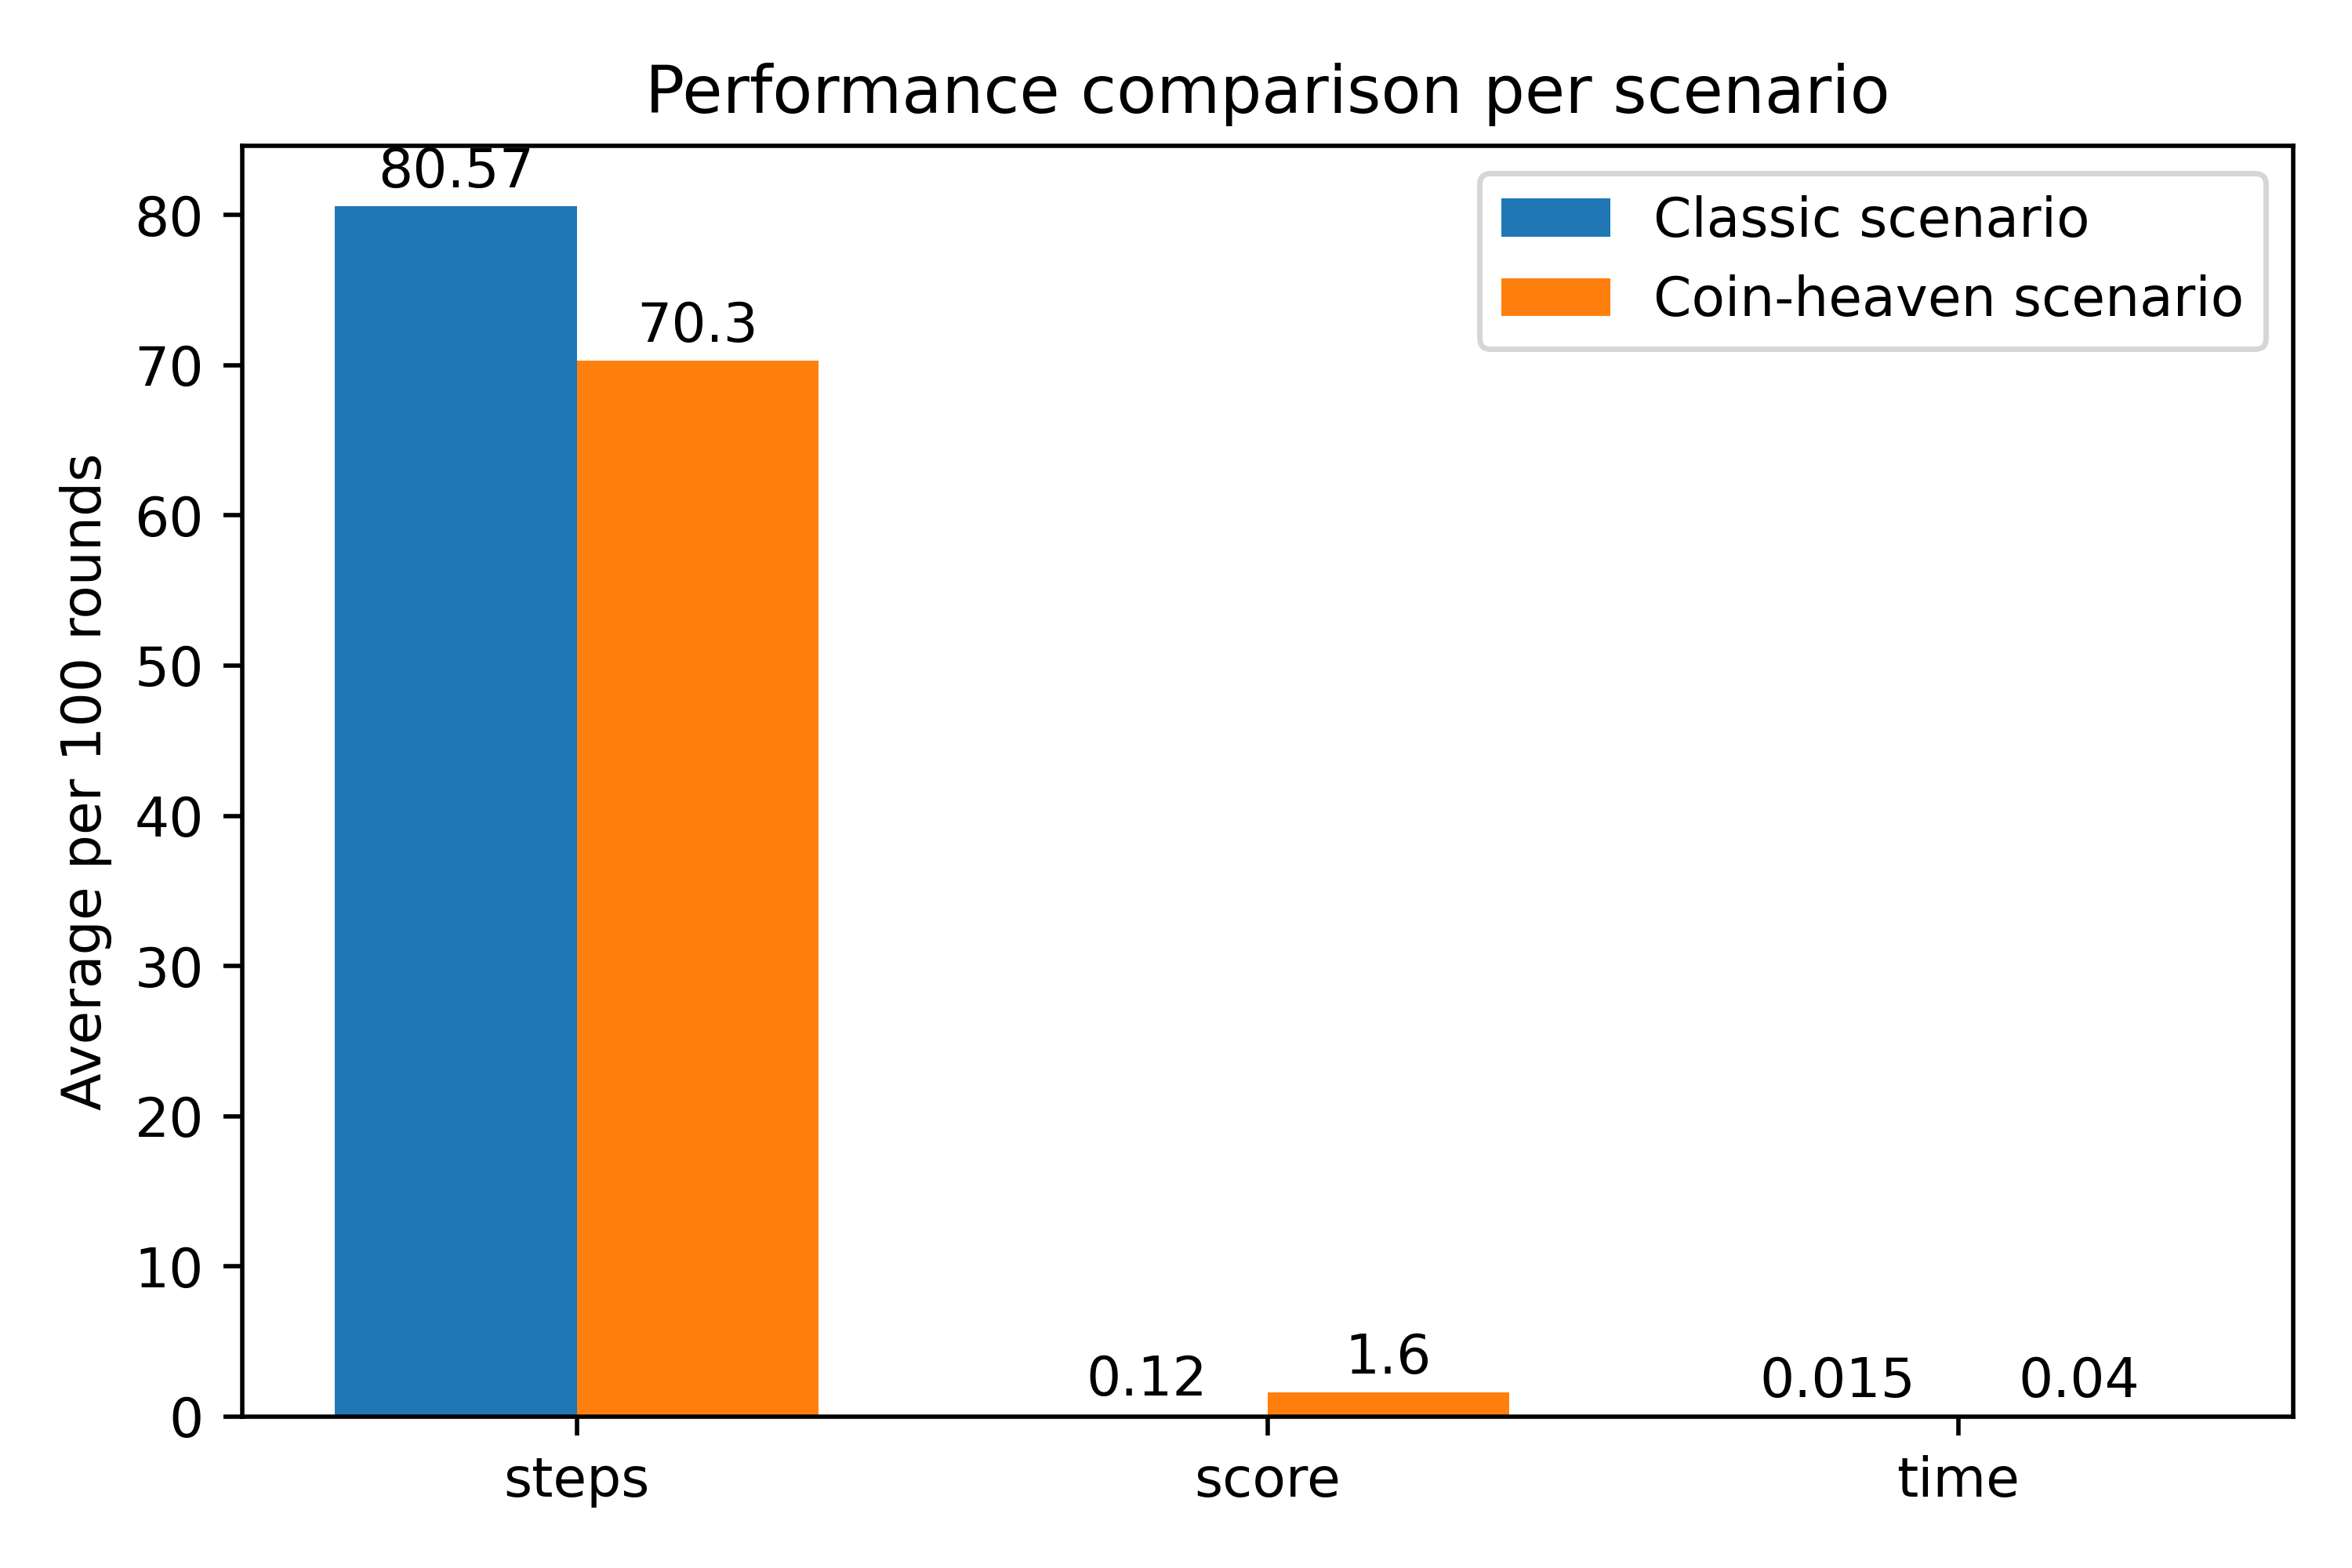
\includegraphics[scale=0.6]{Figures/metrics.png}
	\caption{Comparison of game metrics in the classic and coin-heaven scenario. The values
		correspond to an average value per round after playing for 100 rounds.}
	\label{img:metrics}
\end{figure}

Figure \ref{img:metrics} shows the game metrics in the classic and the coin-heaven
scenario. Each value equals to the average value per round after playing 100 rounds.

In the classic scenario, the agent plays on average for 80 steps. In contrast, in the
coin-heaven scenario the agent plays only for 70 steps. In both scenarios, the
average round ends way before the 400 steps are achieved. The reason lies at that
the use of a dynamic reward shaping function in combination with a high $\gamma$ hyperparameter.
A high $\gamma$ emphasizes future rewards, which incentivizes the agent to collect a high cumulative ?? reward
over the round. However, the dynamic reward shaping function reduces the reward by the time step,
to incentivize the agent to finish the round fast. Therefore, the agent is incentivized to end the
round early to maximize its rewards, which is clearly the case in both scenarios.

In the coin-heaven scenario, the average score equals to 1.6 points which is by 13 times higher.
While in the classic scenario,
the agents earns 0.12 points. As the agent was primarily trained in the coin-heaven scenario, the Q values of
the states of the coin-heaven scenario converged better than the Q values of the classic scenario.

The think time in the coin-heaven scenario is by 2.5 times higher than in the classic scenario.
The think time at seen states is XX??. For unseen states, the agent searches for the most similar seen state
in the Q table and chooses its best action. ????


\begin{figure}[h]
	\centering
	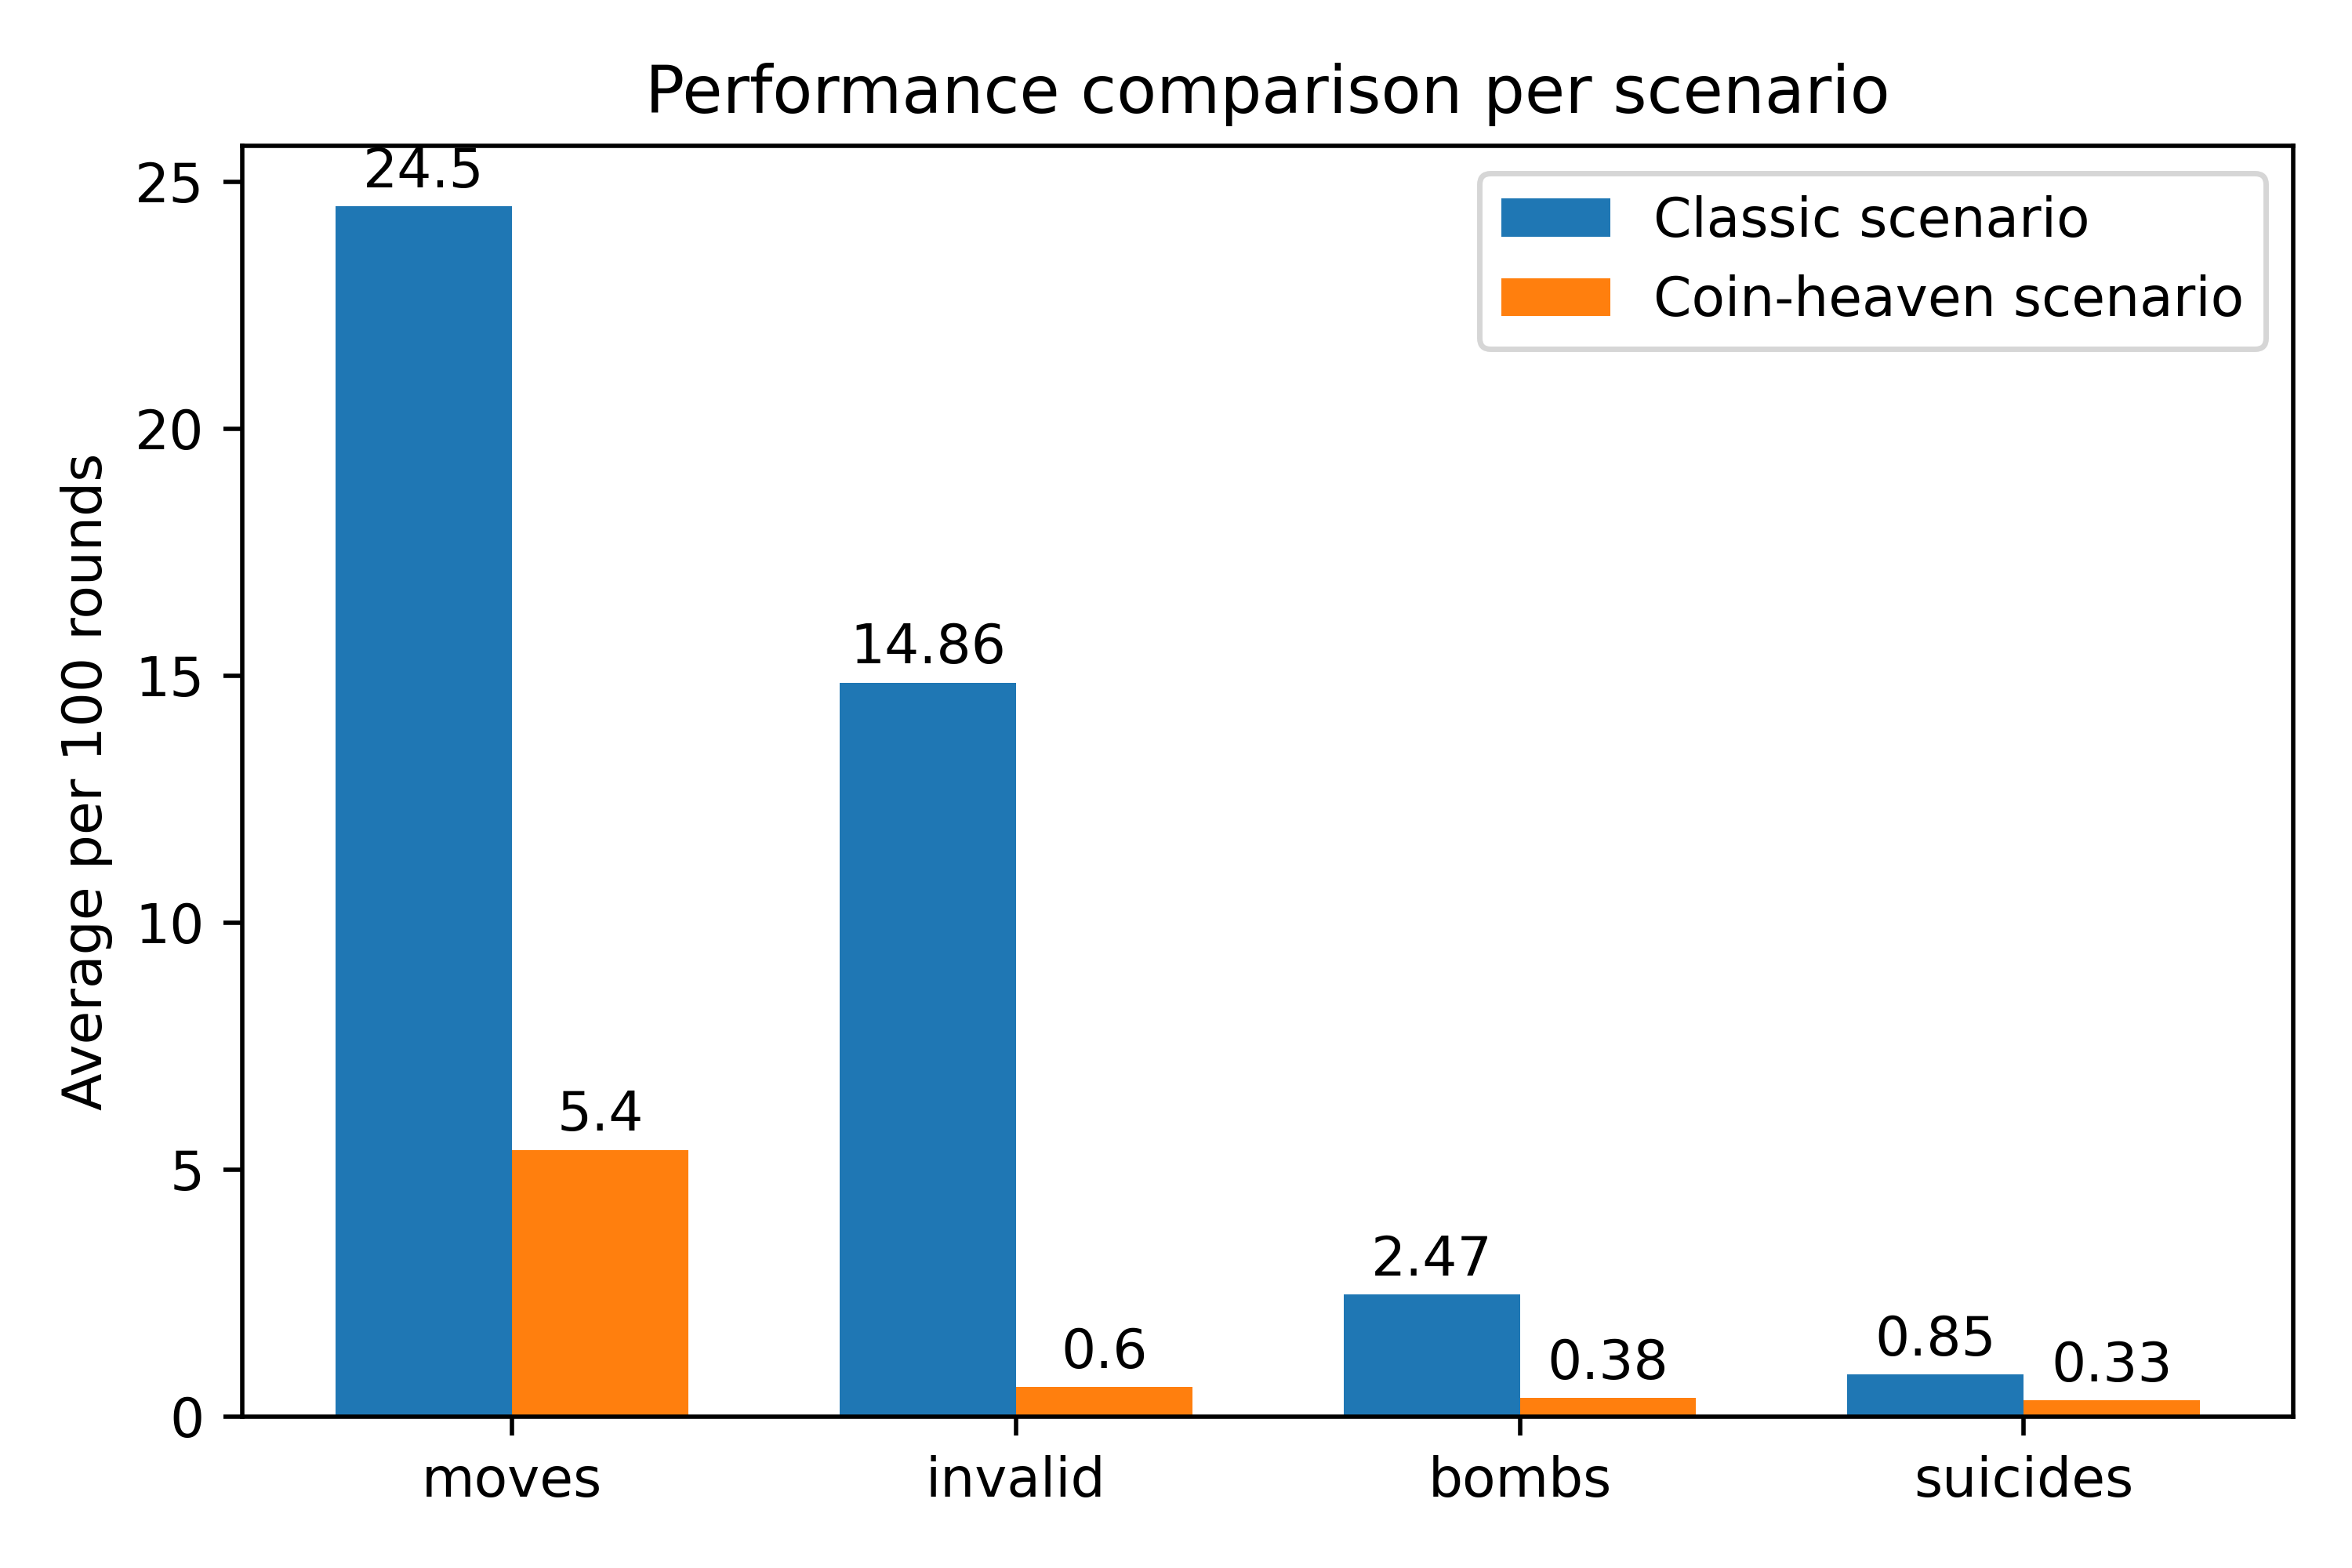
\includegraphics[scale=0.6]{Figures/game.png}
	\caption{Comparison of performance in the classic and coin-heaven scenario. The values
		correspond to an average value per round after playing for 100 rounds.}
	\label{img:game}
\end{figure}

Figure \ref{img:game} shows the effect of the moves in the classic and the coin-heaven
scenario.


Over all four metrics the classic scenario contains consistently higher values.
This indicates the worst performance in comparison to the coin-heaven scenario, which
aligns with our focus on training in the coin-heaven scenario.
This observation becomes even more obvious when considering bad actions such as invalid actions and suicides.
In the coin-heaven scenario the agent chooses on average 24 times more invalid actions and performs 2.5 times
more suicides.

In the classic scenario, as the agent is less cautious with its moves, its performs on average 24.5 moves per round.
The ratio is 5x.???? what are moves

Surprisingly, the agent places 6 times more bombs in the classic scenario. Despite the shorter training time,
the beneficial action is selected way more times than in the coin-heaven scenario. Given that there are less
crates and opponents in the coin-heaven scenario than in the classic scenario, the auxilliary rewards incentivized
the use of bombs in the classic scenario. While 2.4 bombs are certainly not enough to win the round,
the bomb ratio between the two scenarios shows that the rewards give the right incentives. The main issue remains
the long training time until convergence.


Overall, the agent shows better performance in the coin-heaven scenario than in
the classic scenario. The performance is consistently better over all metrics except the time.
The longer training time resulted into more Q values closer to convergence. Nevertheless,
we observe good behavior in both scenarios, such as a low number of invalid actions and more bombs placing in
the scenario with crates and opponents.


%----------------------------------------------------------------------------------------
%	CONCLUSION
%----------------------------------------------------------------------------------------

\section{Conclusions}


\subsection*{Q-Learning}

%----------------------------------------------------------------------------------------
%	BIBLIOGRAPHY
%----------------------------------------------------------------------------------------

\printbibliography % Output the bibliography

%----------------------------------------------------------------------------------------

\end{document}